\section{modélisation de la base de données}
la modélisation de la base de données c'est fait progressivement tout au long du stage. Chaque fois on essayait de l'améliorer en y apportant les ajouts nécessaire pour la faire correspondre à l'idée de départ d'une base de données générique. Au moment de la rédaction du rapport, sa modélisation n'est pas encore fini ou plutôt n'est pas encore validé. Toute fois, nous avons décidé d'y insérer des données et la testée jusqu'à ce qu'à ce que nous rencontrions un problème. Si un problème apparaît alors nous essaierons de l'améliorer encore.

\subsection{Principe d'une base de données générique}
D'une manière générale, lorsqu'on modélise une base de données, on regroupe entre eux les objets ayant les mêmes propriétés dans entités. Ainsi par exemple pour une base de données qui stocke des objets de type moutons et voitures, on aura des entités(tables) moutons et voiture comme dans l'exemple qui suit : 

\begin{figure}[h!]
\begin{center}
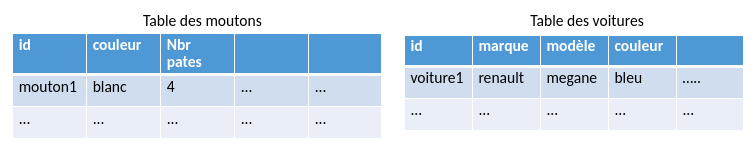
\includegraphics[width=1\textwidth]{images/bd_image1.png}
\end{center}
\caption{exemples de tables d'une base de données}
\label{exemples de tables d'une base de données}
\end{figure}

la modélisation devient d'autant plus difficile si dès le départ on ne connaît pas l'ensemble des objets que l'on doit stocker. En d'autres mots, on souhaite faire une base de données pour contenir plusieurs type d'objets dont les propriétés ne sont pas connu à l'avance. Dans l'exemple ci-dessus, ça correspondrait à stoker, en plus des moutons et des voitures, des immeubles, des personnes et tout autre type d'objet. Pour y remédier, on fait intervenir les bases de données générique. Cela consiste modifier la structure de notre entité et la faire correspondre à une système proche du schéma (clé:valeur). Ce cas de figure fait passer les propriétés des entités dans les colonnes.
l'exemple ci-dessous illustre bien ces propos

\begin{figure}[h!]
    \begin{center}
         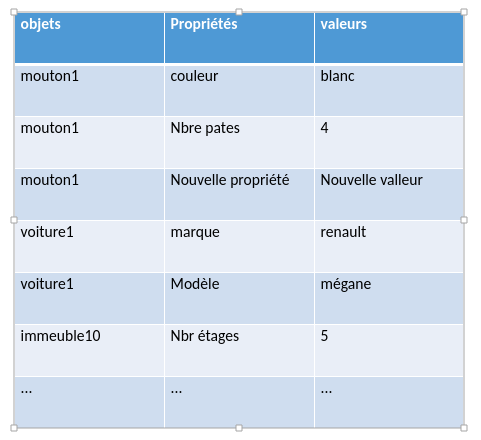
\includegraphics[width=0.4\textwidth]{images/bd_image2.png}
    \caption{exemple de table d'une base de données générique}
    \label{exemple de table d'une base de données générique}
    \end{center}
\end{figure}



% image de la base de données
\begin{landscape}
\begin{figure}
   \begin{center}
       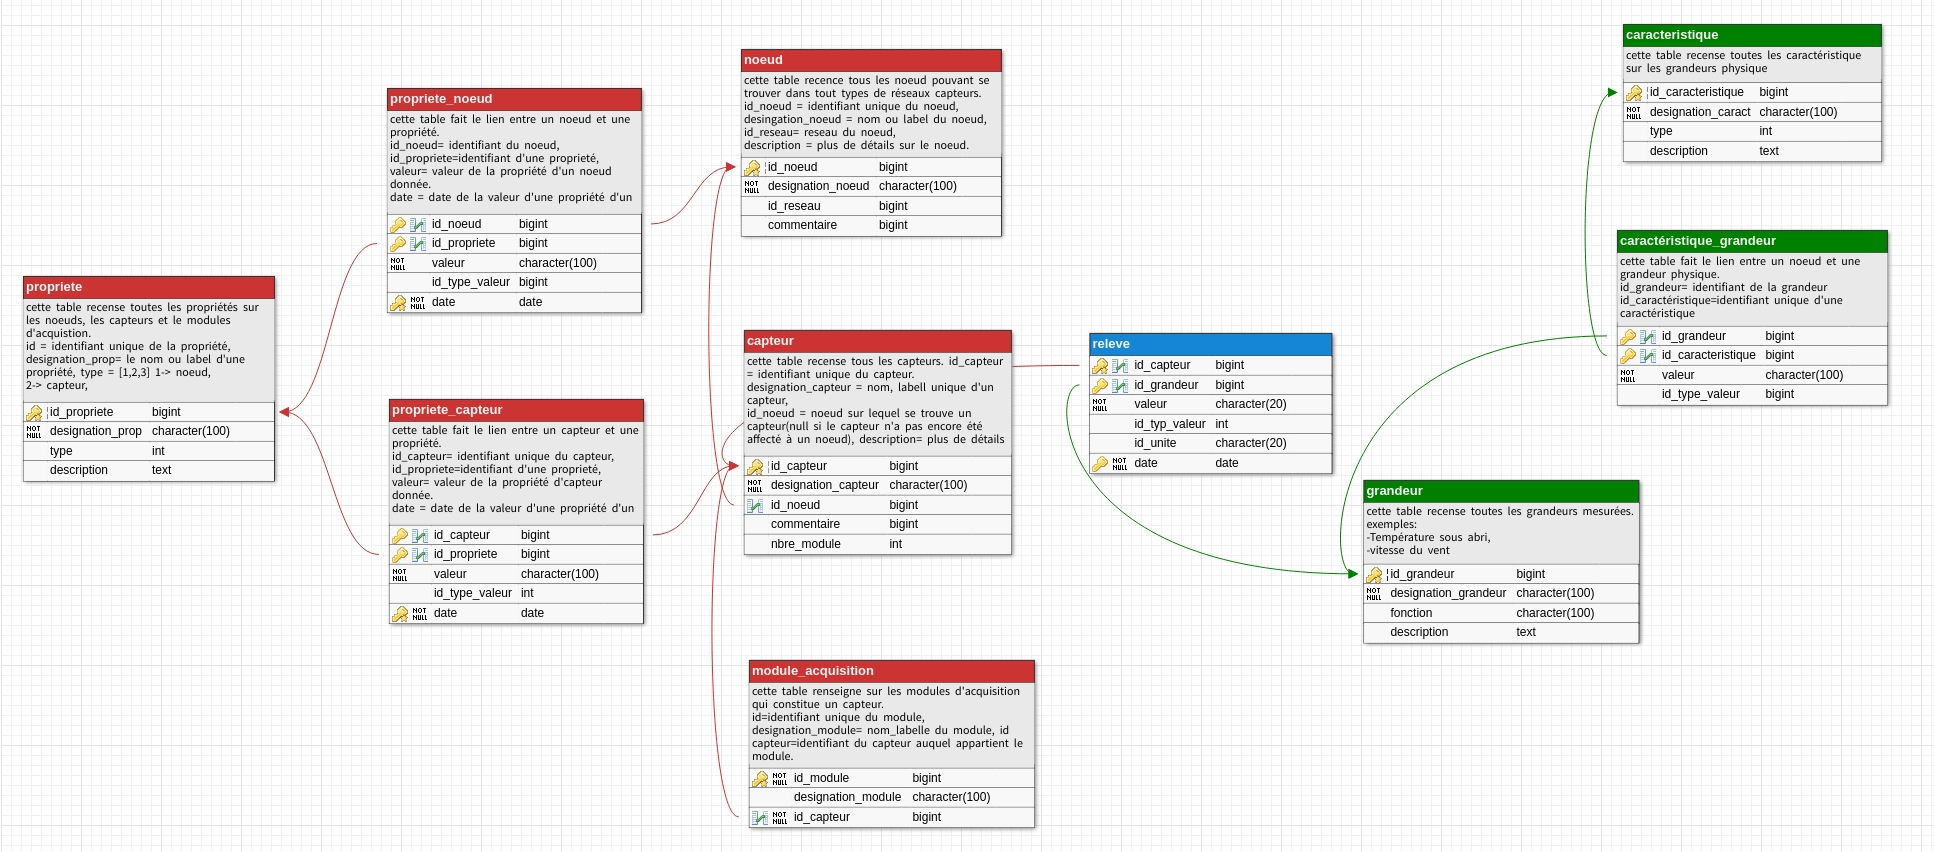
\includegraphics[width=1.8\textwidth]{images/bd_image3.jpg}
    \caption{Caption}
    \label{fig:my_label}
   \end{center}
\end{figure}
\end{landscape}

